\NeedsTeXFormat{LaTeX2e}
\listfiles
\setcounter{errorcontextlines}{\maxdimen}
\documentclass{beamer}
\setbeamercolor{postitlightlightgreen}{fg=Mittel-Blau,bg=green!30}

\usepackage{tabitem-beamer}
\newcommand{\Mittelblau}[1]{\textcolor{Mittel-Blau}{#1}}
%\input{build/Config}
\def\LectureLanguage{eng}
\def\LectureProgLanguage{python}
\def\LectureDesign{ufcd}
%%%%%%%%%%%%%%%%%%

\usepackage{mathtools, amsmath}

\usepackage[binary-units=true]{siunitx}
\usepackage{units}

\usepackage{adjustbox}

\usepackage{tabularx, colortbl, booktabs} % Tables

\usepackage{tikz}
\usepackage{pgfplots}
\usetikzlibrary{patterns,arrows,decorations.pathreplacing,shapes.geometric, 
backgrounds, calc}

\usepackage{wasysym} % Checkmark etc.

\usepackage{listings} % Code
\input{Styles/Code/listings-python.prf} % Python style

%See:
%http://tex.stackexchange.com/questions/280598/simpler-way-to-add-color-to-equations-in-math-mode
\def\mathcolor#1#{\@mathcolor{#1}}
\def\@mathcolor#1#2#3{\protect\leavevmode\begingroup\color#1{#2}#3\endgroup}
\input{Packages/LecturePackages_\LectureLanguage}

\usepackage{ufcd}

\def\PresentationLectureNumber{5}
\def\PresentationExerciseFeedback{false}% Include the feedback of the exercises?
\def\PresentationLectureFeedback{false}% Include the feedback of the lecture?

\def\PresentationDate{November~2017}

\def\PresentationAuthor{Prof.\ Dr.\ Rolf\ Backofen}
\def\PresentationAuthorText{Prof.~Dr.~Rolf~Backofen}

\input{Settings/LectureSettings_\LectureLanguage}

\addtobeamertemplate{navigation symbols}{}{%
    \usebeamerfont{footline}%
    \usebeamercolor[fg]{footline}%
    \hspace{1em}%
    \insertframenumber/\inserttotalframenumber
}

\title[beamer-plain]{\PresentationTitle}
\subtitle{\PresentationDescription}
\author[\PresentationAuthor]{\PresentationAuthorText}
\institute[\PresentationInstitute]{\PresentationInstituteText}
\date[\PresentationDate]{\PresentationSmallTitle, \PresentationDate}

\colorlet{MainA}{blue}
\colorlet{MainALight}{blue!50!white}
\colorlet{Mittel-Blau}{blue!50!white}
\colorlet{Hell-Gruen}{green!50!white}
\colorlet{Mittel-Gruen}{green!50!white}
\colorlet{pgffillcolor}{blue!50!white}

\colorlet{MainADark}{blue!70!black}

\colorlet{MainB}{green}
\colorlet{MainBLight}{green!50!white}
\colorlet{MainBDark}{green!70!black}

\colorlet{SecA}{red!70!black}
\colorlet{SecALight}{red!50!white}
\colorlet{SecADark}{red}

\colorlet{SecB}{orange}
\colorlet{SecBLight}{yellow}
\colorlet{SecBDark}{orange!80!red!60!black}

% Alternative: Anthrazit // Mittel-Grau
\colorlet{Hint}{white!60!black}


\usepackage[autostyle=true]{csquotes}
\usepackage{ifthen}

% We need topics for our sources for grouping
% old: \usepackage[backend=bibtex]{biblatex}
\usepackage[defaultbib]{bibtopic}
\bibliographystyle{alpha}
\renewcommand{\thebtauxfile}{\jobname.\arabic{btauxfile}.btaux}

%%% Source of eatdot
%%%http://tex.stackexchange.com/questions/152892/how-to-delete-a-full-stop-on-reference-ending
\newcommand\eatdot[1]{}

%%% Source of subtoc-fix
%%% 
%%%http://stackoverflow.com/questions/2795478/latex-beamer-prevent-showing-the-toc-at-one-occation
\newboolean{sectiontoc}
\setboolean{sectiontoc}{true} % default to true
\newcommand{\toclesssection}[1]{
  \setboolean{sectiontoc}{false}
  \section{#1}
  \setboolean{sectiontoc}{true}
}

\newboolean{subsectiontoc}
\setboolean{subsectiontoc}{true} % default to true
\newcommand{\toclesssubsection}[1]{
  \setboolean{subsectiontoc}{false}
  \subsection{#1}
  \setboolean{subsectiontoc}{true}
}

\ifthenelse{\equal{\LectureProgLanguage}{all}}{%
  \newcommand{\codeslide}[2]{#2}%
}{%
  \newcommand{\codeslide}[2]{%
    \ifthenelse{\equal{#1}{\LectureProgLanguage}}{#2}{}%
  }%
}%

\AtBeginSection[]
{
  \ifthenelse{\boolean{sectiontoc}}{
    \begin{frame}<beamer>{\LectureToC}
      \tableofcontents[currentsection]
    \end{frame}
  }
}

\AtBeginSubsection[]
{
  \ifthenelse{\boolean{subsectiontoc}}{
    \begin{frame}<beamer>{\LectureToC}
      \tableofcontents[currentsection,currentsubsection]
    \end{frame}
  }
}

\begin{document}

\begin{frame}
  \titlepage
\end{frame}

\begin{frame}{\LectureToC}
  \tableofcontents
  % Die Option [pausesections] k"onnte n"utzlich sein.
\end{frame}

\ifthenelse{\boolean{\PresentationLectureFeedback}}{
  \ifthenelse{\boolean{\PresentationExerciseFeedback}}{
    \section{\LectureFeedbackSection}
  }{}
}{}

\ifthenelse{\boolean{\PresentationExerciseFeedback}}{
  \toclesssubsection{\LectureFeedbackExercisesSection}
  \input{Feedback/FeedbackExercises_\LectureLanguage}
}{}

\ifthenelse{\boolean{\PresentationLectureFeedback}}{
  \toclesssubsection{\LectureFeedbackLectureSection}
  \input{Feedback/FeedbackLecture_\LectureLanguage}
}{}

%%%%\input{build/Chapters_\LectureLanguage}
%-------------------------------------------------------------------------------

\begin{frame}{Runtime analysis - Minsort 1/10}
  \begin{center}
    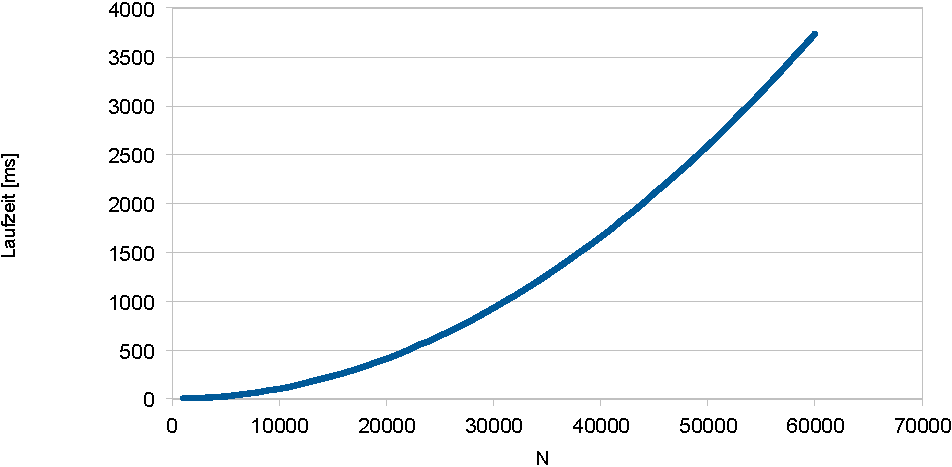
\includegraphics[width=0.65\textwidth]{Rolfs-Images/runtime-minsort.pdf}
  \end{center}
 How long does the program run?
 \begin{itemize}
    \item
      In the last lecture we had a schematic.
    \item
      \textbf{Observation:} It is going to be \enquote{disproportional} slower
      the more numbers are being sorted.
    \item
      How can we say more precisely what is happening?
  \end{itemize}
\end{frame}

%-------------------------------------------------------------------------------
\begin{frame}{Runtime analysis - Minsort 2/10}
  How can we analyse the runtime?
  \begin{itemize}
    \item Ideally we have a formula which provides the runtime of the
      program for an specific input
    \item
      \textbf{Problem:} The runtime is also depending on many other
        influences, especially:
      \begin{itemize}
        \item
          Which kind of computer is the code executed on.
        \item What is running in the background.
        \item Which compiler is used to compile the code.
      \end{itemize}
    \item
      \textbf{Abstraction 1:} Analyse the number of basic operations,
        rather than analysing the runtime.
  \end{itemize}
\end{frame}

\begin{frame}{Basic Operations}
  Uncomplete list of basic operations
  \begin{center}
    \begin{itemize}
      \item
        arithmetic operation, for example: \textit{a + b}
      \item
        allocation of variables, for example: \textit{x = y}
      \item 
        function call, for example: \textit{Sorter.minSort(array)}
    \end{itemize}
  \end{center}
\end{frame}

%-------------------------------------------------------------------------------

\begin{frame}{Basic Operations}
  \begin{tabularx}{\textwidth}{@{}XcXcX@{}}
    \cellcolor{Mittel-Blau} {\color{white}\textbf{Intuitive:}} &
    {} &
    \cellcolor{Mittel-Blau} {\color{white}\textbf{Better:}} &
    {} &
    \cellcolor{Mittel-Blau} {\color{white}\textbf{Best:}}\\[0.5em]
    \rule{0pt}{1.25em}\cellcolor{Hell-Blau}lines of code &
    {} &
    \cellcolor{Hell-Blau}lines of machine code &
    {} &
    \cellcolor{Hell-Blau}process cycles
  \end{tabularx}\\[1.5em]
  \begin{alertblock}{\textbf{Important:}}
    The actual runtime has to be roughly proportional
    to the number of operations.
  \end{alertblock}
\end{frame}\section{Runtime Example}

\begin{frame}{Runtime analysis - Minsort 3/10}
  How many operations does \textit{Minsort} need?
  \begin{itemize}
    \item
      \textbf{Abstraction 2:} We calculate the upper (lower) bound,
      rather than counting the operations exactly.

      \textbf{Reason}: Runtime is unknown, but we know:
      \begin{itemize}
        \item {\color{Hell-Gruen}upper bound}
        \item {\color{Hell-Gruen}lower bound}
      \end{itemize}
    \item \textbf{Basic Setting}
      \begin{tabl}
      \item \Mittelblau{$n$} is size of input (i.e., array)
      \item \Mittelblau{$T(n)$} number of operations for input $n$
      \end{tabl}
    \item
      \textbf{Observation:} The number of operations needed is only
      depending on the size {\color{Mittel-Blau}$n$} of the array and not on the content!
    \item \textbf{Claim:} There are constants \Mittelblau{$C_1$} and
      \Mittelblau{$C_2$} such that
      \begin{displaymath}
        \color{Mittel-Blau}C_1\cdot n^2 \leq T(n) \leq        C_2\cdot n^2 
      \end{displaymath} \vspace*{-2em}
    \item this is called ``quadratic runtime''  (due to \Mittelblau{$n^2$})
  \end{itemize}
\end{frame}

%-------------------------------------------------------------------------------

\begin{frame}{Runtime Example}
  \begin{figure}[!h]
    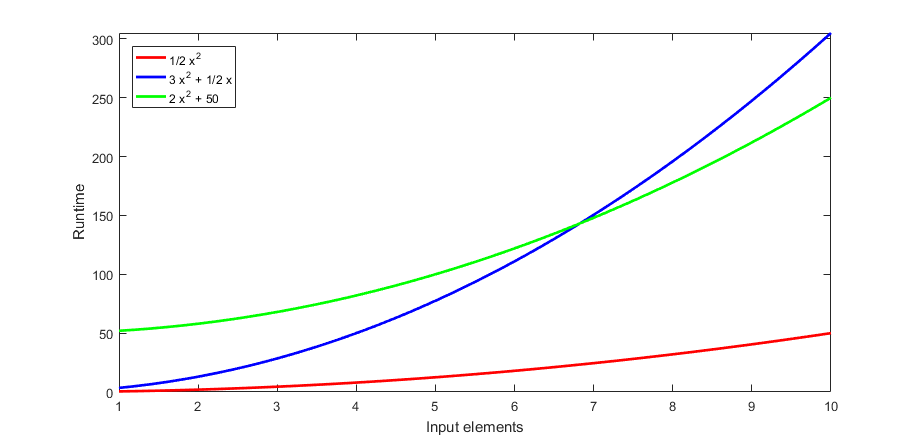
\includegraphics[width=\linewidth]
      {Images/Runtime/SquaredRuntime.png}%
    \caption{Different functions with quadratic runtime}%
    \label{fig:squared_runtime}%
  \end{figure}
\end{frame}

%-------------------------------------------------------------------------------

\subsection{Minsort \ldots{}``quadratic Runtime''}


\begin{frame}{Runtime analysis - Minsort 4/10}
  \textbf{We declare:}
  \begin{itemize}
    \item Runtime of operations: $T(n)$
    \item Number of Elements: $n$
    \item Constants: $C_1$ ({\color{Hell-Gruen}lower bound}),
      $C_2$ ({\color{Hell-Gruen}upper bound})
    \begin{center}
      $C_{1} \cdot n^2
      \leq T(n)
      \leq C_{2} \cdot n^2$
    \end{center}
    \item Number of operations in round $i$: $T_i$
  \end{itemize}
  \begin{figure}[!h]
    \begin{adjustbox}{width=0.5\linewidth}
      \def\AlgoMinsort#1#2#3{
  \draw[fill=#3] (#1 + 0.1, 0.0) rectangle (#1 + 0.9, #2/2);
  \draw (#1 + 0.5, -0.5) node {\huge #2};
}
\begin{tikzpicture}
%Generate MinSort pattern
\foreach[count=\x] \h/\c in {
  1/MainBLight,%
  2/MainBLight,%
  3/MainBLight,%
  12/MainALight,%
  7/MainALight,%
  4/MainA,%
  6/MainALight,%
  10/MainALight,%
  8/MainALight,%
  15/MainALight,%
  14/MainALight,%
  5/MainALight,%
  11/MainALight,%
  9/MainALight,%
  13/MainALight%
} {
  \AlgoMinsort{\x}{\h}{\c}
}
\end{tikzpicture}%
    \end{adjustbox}%
    \caption{\textit{Minsort} at the fourth iteration}%
    \label{fig:minsort_def}%
  \end{figure}
\end{frame}
%-------------------------------------------------------------------------------

\begin{frame}{Runtime analysis - Minsort 5/10}
  \begin{columns}
    \begin{column}{0.55\textwidth}
      \begin{figure}[!h]%
        \begin{adjustbox}{width=\linewidth}%
          \def\MinSortDrawNumbers{0}
\begin{tikzpicture}
%Generate MinSort pattern
\foreach[count=\x] \h/\c in {
  1/MainBLight,%
  2/MainBLight,%
  3/MainBLight,%
  12/MainALight,%
  7/MainALight,%
  4/MainA,%
  6/MainALight,%
  10/MainALight,%
  8/MainALight,%
  15/MainALight,%
  14/MainALight,%
  5/MainALight,%
  11/MainALight,%
  9/MainALight,%
  13/MainALight%
} {
  \draw[fill=\c] (\x + 0.1, 0.0) rectangle (\x + 0.9, \h/2);
  \ifnum \MinSortDrawNumbers>0
    \draw (\x + 0.5, -0.5) node {\huge \h};
  \fi
}

%Draw brace
\draw (4.0, 7.5)
  [
    line width=0.25em,
    color=black,
    decoration={
        brace,
        raise=0.75em,
        amplitude=15pt
    },
    decorate
  ] --
  node [
    color=black,
    pos=0.5,
    yshift=4em,
    font=\Huge
  ] {$n-3$ elements left}
  (16.0, 7.5);
\end{tikzpicture}%
        \end{adjustbox}%
        \caption{\textit{Minsort} at the fourth iteration}%
        \label{fig:minsort_brace}%
      \end{figure}
    \end{column}
    \begin{column}{0.40\textwidth}
      Compares at each iteration:
      \begin{align*}
        T_1  \leq &~ n\\
        T_2  \leq &~ (n-1)\\
        {}  \vdots~ &~ {} \\
        T_{n-1}  \leq &~ 2\\
        T_n  \leq &~ 1
      \end{align*}
    \end{column}
  \end{columns}
  \[
    T(n)
      = C \cdot \left(T_1 + \cdots + T_n\right)
      \leq C \cdot \sum \limits^n_{i=1} i
  \]
\end{frame}

%-------------------------------------------------------------------------------

\begin{frame}{Runtime Example}
  \begin{itemize}
    \item
      The runtime is growing quadratic with the number of elements
      ${\color{Mittel-Blau}n}$ in the list.\\
    \item
      $2\, \times$ elements $\Rightarrow$ $4\, \times$ runtime\\
      \begin{itemize}
        \item 
          $C = \SI{1}{\nano\second}$
          (1 simple instruction $\approx \SI{1}{\nano\second}$)
        \item 
          $n = 10^6$ (1 million numbers = $\SI{4}{\mega\byte}$
          with $\SI{4}{\byte\per number}$)
          \begin{itemize}
            \item 
              $C \cdot n^2 = \SI{e-9}{\second} \cdot 10^{12}
               = \SI{e3}{\second} = \SI{16.7}{\minute}$
          \end{itemize}
        \item 
          $n = 10^9$ (1 billion numbers = $\SI{4}{\giga\byte}$)
          \begin{itemize}
            \item 
              $C \cdot n^2 = \SI{e-9}{\second} \cdot 10^{18}
               = \SI{e9}{\second} = 31.7$~years
          \end{itemize}
      \end{itemize}
    \item
      \textbf{Quadratic runtime = \enquote{big} problems unsolvable}
  \end{itemize}
\end{frame}\toclesssection{Runtime analysis}






%-------------------------------------------------------------------------------

% \codeslide{python}{
% \begin{frame}{Runtime analysis - Minsort 6/10}
%   \textbf{Alternative: Analyse the Code:}
%   \lstinputlisting[
%     language=Python,
%     style={python-idle-code},
%     basicstyle=\small,
%     tabsize=4,
%     emph={minsort},
%     emphstyle=\color{blue}
%   ]{Code/MinSort.py}
% \end{frame}
% }
% %TODO: MinSort Java, C++

\begin{frame}{Runtime analysis - Minsort 6/10}
  \begin{tabl}
  \iitem{-2em}
\onslide<1>{\rlap{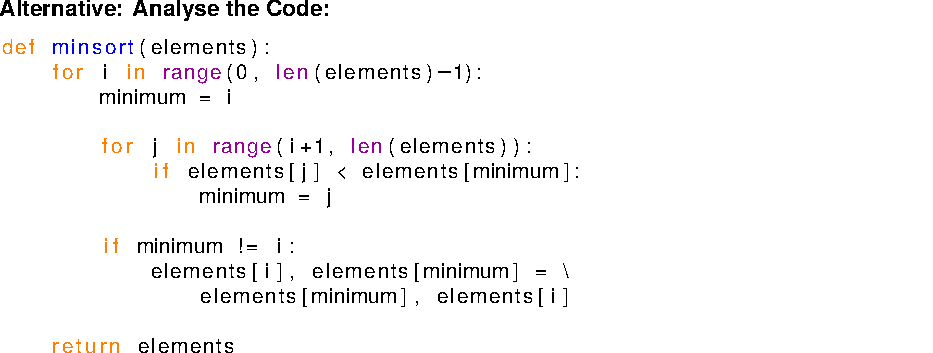
\includegraphics[width=1.15\textwidth]{Rolfs-Images/minsort-code-analysis-o1.pdf}}}%
\onslide<2>{\rlap{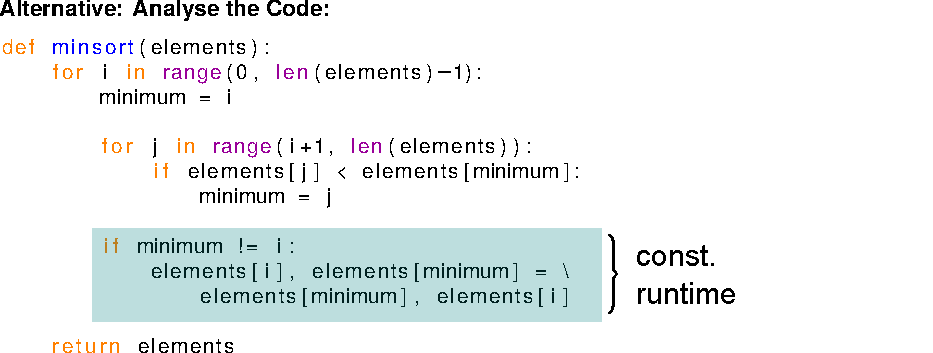
\includegraphics[width=1.15\textwidth]{Rolfs-Images/minsort-code-analysis-o2.pdf}}}%
\onslide<3>{\rlap{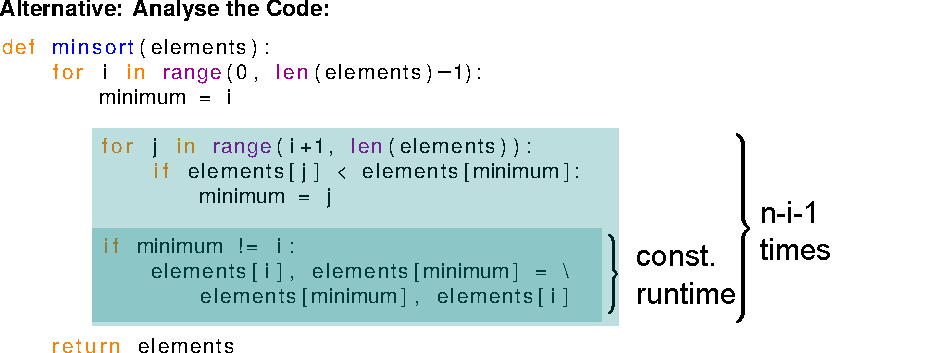
\includegraphics[width=1.15\textwidth]{Rolfs-Images/minsort-code-analysis-o3.pdf}}}%
\onslide<4->{\rlap{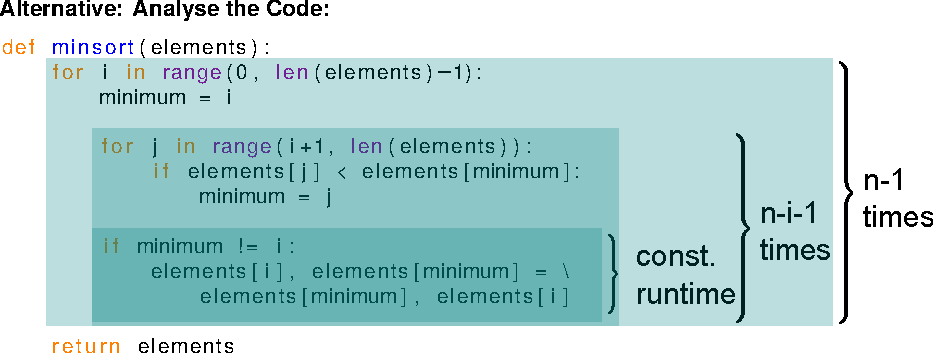
\includegraphics[width=1.15\textwidth]{Rolfs-Images/minsort-code-analysis-o4.pdf}}}%
  \end{tabl}
  \vspace*{-1em}
\begin{displaymath}
\color{Mittel-Blau}
\onslide<5-> T(n)  \leq \sum^{n-2}_{i=0}
\sum^{n-1}_{j=i+1} C'_2 
\onslide<6-> = \sum^{n-2}_{i=0} (n-i-1)\cdot C'_2
\onslide<7-> = \sum^{n-1}_{i=1} (n-i)\cdot C'_2 
\onslide<8-> \leq \sum^{n-1}_{i=1} i\cdot C'_2 
\end{displaymath}
\vspace*{-2em}\onslide<9-> \textbf{Remark} $C'_2:$ cost of swap
operation $\Rightarrow$ assumed constant\vspace*{2em}
\end{frame}


%-------------------------------------------------------------------------------

% \begin{frame}{Runtime analysis - Minsort 7/10}
%   \begin{center}
%     \begin{math}
%       \begin{array}{l}
%         \displaystyle
%         \max T(n) = \underbrace{
%           \sum^{n - 2}_{i = 0}
%           \left(
%             \hspace*{1.5em}
%             \overbrace{
%               C'_2
%               \vphantom{
%                 \sum^{n - 1}_{j = i + 1}
%               }
%             }^\text{swap}
%             \hspace*{1.5em} +
%             \underbrace{
%               \overbrace{
%                 \hspace*{0.5em}
%                 \sum^{n - 1}_{j = i + 1} C'_1
%                 \hspace*{0.5em}
%               }^\text{compare}
%             }_{
%             \lstinline[
%               language=Python,
%               style={python-idle-code},
%               basicstyle=\small
%               ]|range(i+1, len(elements))|
%             }
%             \hspace*{0.5em}
%           \right)
%         }_{
%         \lstinline[
%           language=Python,
%           style={python-idle-code},
%           basicstyle=\small
%         ]|range(0, len(elements)-1)|
%       }\\[5em]
%       \displaystyle\hspace*{2.5em}
%         = \sum^{n - 2}_{i = 0} \left(C'_2 + (n - i) C'_1\right)\\
%       \displaystyle\hspace*{2.5em}
%         = \color{Mittel-Blau}
%         \sum^{n - 1}_{i = 1} \left(C'_2 + (n - i + 1) C'_1\right)
%       \end{array}
%     \end{math}
%   \end{center}
% \end{frame}

% %-------------------------------------------------------------------------------

% \begin{frame}{Runtime analysis - Minsort 7/10}
%   \begin{center}
%     \begin{math}
%       T(n) \leq
%       \left\lbrace
%       \begin{array}{l}
%       \displaystyle\hspace*{1.5em}\color{Mittel-Blau}
%         \sum^{n - 1}_{i = 1} \left(C'_2 + (n - i + 1) C'_1\right)\\
%       \displaystyle\hspace*{1.5em}
%         = \sum^{n - 1}_{i = 1} \left(C'_2 + C'_1\right)
%         + \sum^{n - 1}_{i = 1} \left(n - i\right) C'_1\\
%       \displaystyle\hspace{1.5em}
%         = \left(n - 1\right) \cdot \left(C'_2 + C'_1\right)
%         + C'_1 \sum_{i = 1}^{n - 1} i\\
%      % \displaystyle\hspace*{1.5em}
%      %   \leq n \left(C'_2 + C'_1\right) + C'_1 \sum^n_{i=1} i
%       \end{array}
%       \right.
%     \end{math}
%   \end{center}
% \end{frame}

% %-------------------------------------------------------------------------------
\begin{frame}{Runtime analysis - Minsort 7/10}
  \begin{tabl}
  \eitem {Proof of the statement ({\color{Mittel-Gruen}upper bound}):} 
    $\displaystyle  T(n) \leq C_2 \cdot n^2, \, C_2 = 1$
    \end{tabl}
\color{Mittel-Blau}
    \begin{eqnarray*}
        T(n) & \leq &           \sum \limits^{n - 1}_{i = 1} C'_2\cdot i \\
        \onslide<2->
& = &           C'_2 \cdot \sum \limits^{n - 1}_{i = 1} i\\
        \onslide<3-> & & { \color{black}\hspace*{1cm} \Downarrow \hspace*{0.5cm} \rlap{\text{Small Gauss sum}}}\\
& = &           C'_2 \cdot \frac{n(n + 1)}{2} \\
        \onslide<4-> & & { \color{black}\hspace*{1cm} \Downarrow
          \hspace*{0.5cm} 1 \leq n}\\
& = &           C'_2 \cdot \frac{n(n +n )}{2} \\
        \onslide<5->
& = &           C'_2 \cdot \frac{2n^2}{2}    \quad     \onslide<6->
=\quad C'_2 \cdot n^2
    \end{eqnarray*}

 \end{frame}

 \begin{frame}
   \frametitle{Excursion: Small Gauss Formula}
 \end{frame}
%-------------------------------------------------------------------------------

 \begin{frame}{Runtime analysis - Minsort 9/10}
   \begin{itemize}
   \item Proof of claim $C_1 \cdot n^2 \leq T(n)$
     \begin{itemize}
     \item Corresponding to the upper boundry, there exists a\\
       a $C_1$ for that holds:\\
       \color{Mittel-Blau}
    \vspace{-0.5cm}
    \begin{eqnarray*}
        T(n) & \leq & \sum \limits^{n - 1}_{i = 1} (n - i) \cdot C'_1 =  \sum \limits^{n - 1}_{i = 1} C'_1 \cdot i\\
        \onslide<2->
        & = &           T (n) \leq C'_1 \cdot \frac{(n -1) \cdot n}{2}\\
        \onslide<3-> & & \color{black} \text{How did we get to } \color{Mittel-Blau} n^2 \text{?}\\
        %\onslide<4-> & \color{black}\hspace*{1cm} \Downarrow \hspace*{0.5cm} & \rlap{n - 1 \gt \frac{n}{2} given n \gt 2  \\
        \onslide<4-> & & { \color{black}\hspace*{1cm} \Downarrow
          \hspace*{0.5cm} n - 1 > \frac{n}{2} \text{given } n > 2}\\
        \onslide<5-> C'_1 \cdot \frac{n \cdot n}{2 \cdot 2}& &\\
        \onslide<6-> \frac{C'_1}{4} \cdot n^2 & &\\
        \onslide<7-> & & \text{Summarized } \frac{C'_1}{4} \cdot n^2 \leq T(n) \leq C'2 \cdot n^2 \\
        \onslide<8-> & & \text{Quadratic runtime proven: } C_1 \cdot n^2 \leq T(n) \leq C_2 \cdot n^2 \\
    \end{eqnarray*}

     \end{itemize}
   \end{itemize}
 \end{frame}
 
%-------------------------------------------------------------------------------

\begin{frame}{Runtime analysis - Minsort 10/10}
  
\end{frame}
%% \begin{frame}{Runtime analysis - Minsort 9/10}
%%   \begin{block}{Proof of $C_1 \cdot n^2 \leq T(n)$
%%       ({\color{Mittel-Gruen}lower bound}):}
%%     We assume: Compare $\in \mathcal{O}(1)$\\
%%     $\hspace{1.5em}\Rightarrow C'_1 = 1, \; C'_2 = 0$\\
%%     \vspace*{0.5em}
%%     Analogous for the {\color{Mittel-Gruen}lower bound}
%%     (no value is swapped), there exists a $C_1$, for that
%%     applys:\\[0.5em]
%%     \begin{centering}
%%       \begin{math}
%%         \begin{array}{@{}rcl@{}}
%%           T(n) & \geq &
%%           \displaystyle
%%           n - 1 + \sum^{n - 1}_{i=1} i
%%           = \frac{n^2 - n}{2} + n - 1
%%           = \frac{n^2 + n}{2} - 1
%%         \end{array}
%%       \end{math}
%%     \end{centering}
%%   \end{block}
%% \end{frame}

%% %-------------------------------------------------------------------------------

%% \begin{frame}{Runtime analysis - Minsort 10/10}
%%   \begin{block}{Proof of $C_1 \cdot n^2 \leq T(n)$:}
%%     \vspace*{0.5em}
%%     \begin{center}
%%       $\displaystyle
%%         T(n) \; \geq \;
%%           = \frac{n^2 + n}{2} - 1
%%       $\\
%%     \end{center}
%%     $T(n)$ is always bigger than / equal to $\frac{1}{2} \cdot n^2$
%%     for $n \geq 2$:\\[1.0em]
%%     $\hspace*{1.5em}\Rightarrow T(n) \geq C_1 \cdot n^2$
%%   \end{block}
%% \end{frame}\subsection{Heapsort $\ldots$ better but also not linear }

%-------------------------------------------------------------------------------
\subsection{Heapsort $\ldots$ better but also not linear }

\begin{frame}{Runtime - Heapsort 1/6}
  \textbf{Intuitive:}
  \begin{itemize}
    \item
      \textbf{Minsort:}
      To determine the minimum value we have to iterate through all the
      unsorted elements.
    \item
      \textbf{Heapsort:}
      The root-element is always the smallest (min-heap).
      We only need to repair a small part of the full tree after an delete
      operation.
  \end{itemize}
  \textbf{Formal:}
  \begin{itemize}
    \item 
      Let T$(n)$ be the runtime for the \textit{Heapsort}
      algorithm with $n$ elements.
    \item
      On the next pages we will proof $T(n) \leq C \cdot n \, \log_2 n$
  \end{itemize}
\end{frame}


\begin{frame}{Runtime - Heapsort 2/6}
  \begin{columns}
    \begin{column}{0.5\textwidth}
      Depth of a binary tree:
      \begin{itemize}
        \item
          \textbf{Depth \textit{d}:}
          longest path through the tree
        \item
          Complete binary tree has $n = 2 \cdot d - 1$ nodes
        \item
          Example: $d = 4$\\
          $\Rightarrow n = 2^4 - 1 = 15$
      \end{itemize}
    \end{column}
    \begin{column}{0.5\textwidth}
      \begin{figure}
        \begin{centering}%
          \tikzstyle{node}=[
  draw,
  circle,
  very thick,
  color=black,
  fill=white,
]%
%
\tikzstyle{node_filled}=[
  draw,
  circle,
  very thick,
  color=black,
  fill=orange!50!yellow
]%
%
\tikzstyle{node_leaf}=[
  draw,
  circle,
  very thick,
  color=black,
  fill=green!50!white,
]%
%
\tikzstyle{path}=[
  draw,
  line width=0.25em,
  color=orange!50!yellow!80!black
]%
%
\tikzstyle{path_normal}=[
  draw,
  very thick,
  color=black
]%
%
\begin{adjustbox}{width=\linewidth}
\begin{tikzpicture}[
  level/.style={
    sibling distance = 10.0em/#1,
    level distance = 3.5em
  }
]
\node [node_filled, label={[anchor=south]above:Root}] (root) {}
child [path_normal] {
  node [node] {}
  child {
    node [node] {}
    child {node [node_leaf, label={[anchor=east]left:Leaves}] {}}
    child {node [node_leaf] {}}
  }
  child {
    node [node] {}
    child {node [node_leaf] {}}
    child {node [node_leaf] {}}
  }
}
child [path] {
  node [node_filled] {}
  child {
    node [node_filled] {}
    child [path_normal] {node [node_leaf] {}}
    child {node [node_filled] {}}
  }
  child [path_normal] {
    node [node] {}
    child {node [node_leaf] {}}
    child {node [node_leaf] {}}
  }
};
\end{tikzpicture}
\end{adjustbox}%
          \caption{Binary tree with 15 nodes}%
          \label{fig:binary_tree}%
        \end{centering}%
      \end{figure}
    \end{column}
  \end{columns}
\end{frame}\subsubsection{Depth of a Tree}


\subsubsection{Introduction to Induction}

\begin{frame}<beamer>{Structure}
  \tableofcontents[currentsection,currentsubsection]
\end{frame}

\begin{frame}{Induction}
  \textbf{Basics:}
  \begin{itemize}
    \item 
      You want to show assumption $A(n)$ is valid $\forall n \in \mathbb{N}$
    \item
      We show induction in two steps:
      \begin{enumerate}
        \item
          \textbf{Induction basis:} we show that our assumption is valid 
          at one point (for example: $n = 1$).
        \item
          \textbf{Induction step:} we show that the assumption is valid for 
          all $n$ (normally one step forward: $n = n + 1$).
      \end{enumerate}
    \item If both has been proven, then \Mittelblau{$A(n)$} holds for
      all natural numbers \Mittelblau{$n$} by \textbf{induction}
  \end{itemize}
\end{frame}

%-------------------------------------------------------------------------------

\begin{frame}{Induction - Example 1}
  \fbox{\begin{minipage}{0.45\linewidth}
  \textbf{Claim}   A \textit{complete} binary tree of depth \Mittelblau{$d$}
has \Mittelblau{$n(d)=2^d-1$} many nodes \end{minipage}
}
\rlap{\begin{minipage}{0.5\linewidth}
  \tikzstyle{node}=[
  draw,
  circle,
  very thick,
  color=black,
  fill=white,
]%
%
\tikzstyle{node_filled}=[
  draw,
  circle,
  very thick,
  color=black,
  fill=orange!50!yellow
]%
%
\tikzstyle{node_leaf}=[
  draw,
  circle,
  very thick,
  color=black,
  fill=green!50!white,
]%
%
\tikzstyle{path}=[
  draw,
  line width=0.25em,
  color=orange!50!yellow!80!black
]%
%
\tikzstyle{path_normal}=[
  draw,
  very thick,
  color=black
]%
%
\begin{adjustbox}{width=\linewidth}
\begin{tikzpicture}[
  level/.style={
    sibling distance = 10.0em/#1,
    level distance = 3.5em
  }
]
\node [node_filled, label={[anchor=south]above:Root}] (root) {}
child [path_normal] {
  node [node] {}
  child {
    node [node] {}
    child {node [node_leaf, label={[anchor=east]left:Leaves}] {}}
    child {node [node_leaf] {}}
  }
  child {
    node [node] {}
    child {node [node_leaf] {}}
    child {node [node_leaf] {}}
  }
}
child [path] {
  node [node_filled] {}
  child {
    node [node_filled] {}
    child [path_normal] {node [node_leaf] {}}
    child {node [node_filled] {}}
  }
  child [path_normal] {
    node [node] {}
    child {node [node_leaf] {}}
    child {node [node_leaf] {}}
  }
};
\end{tikzpicture}
\end{adjustbox}
\end{minipage}}
%
\begin{tabl}
\item<2-> \textbf{Induction basis:} formula holds for \Mittelblau{$d=1$}
\sitem 
\citem 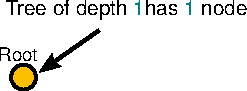
\includegraphics[width=0.45\textwidth]{Rolfs-Images/tree-one-node.pdf}
\eitem
\citem \onslide<3->  \Mittelblau{$n(1) = 2^1 -1 = 1$}\qquad{} correct!
\end{tabl}
\end{frame}

\subsubsection{Depth of a Tree}

\begin{frame}{Induction - Example 1}
  Number of nodes $n(d)$ in a binary tree with depth $d$:
  \begin{itemize}
    \item
      \textbf{Induction assumption:}
      $n(d) = 2^d-1$
    \item
      \textbf{Induction basis:}
      $n(1) = 2^d - 1 = 2^1 - 1 = 1 ~{\color{Mittel-Blau}\checked}$
    \item
      \textbf{Induction step:}
      to show for $d = d + 1$
      \begin{columns}
        \begin{column}{0.6\textwidth}
          \begin{figure}%
            \begin{centering}%
              \begin{tikzpicture}[
  level/.style={
    sibling distance = 8.0em,
    level distance = 1.5em
  },
  node/.style={
    draw,
    circle,
    very thick,
    color=black,
    fill=white
  },
  node_tree/.style={
    node,
    color=black,
    fill=white
  },
  node_filled/.style={
    node,
    color=black,
    fill=orange!50!yellow
  },
  tree/.style={
    draw,
    very thick,
    shape border uses incircle,
    isosceles triangle,
    shape border rotate=90,
    yshift=-4em,
    color=black,
    fill=green!50!white,
    minimum height=8.0em
  },
  path/.style={
    draw,
    very thick,
    color=black
  },
  brace/.style={
    very thick,
    color=black,
    decoration={
      brace,
      raise=0.75em,
      amplitude=15pt
    },
    decorate
  },
  line/.style={
    draw,
    loosely dotted,
    very thick,
    color=black
  }
]%
\node [node_filled, label={[anchor=south]above:Root}] (root) {}
child [path] {
  child {
    node[tree] {\only<4->{\Large $v(d)$}}
  }
  node [node_tree] {}
}
child [path] {
  child {
    node[tree] {\only<4->{\Large $v(d)$}}
  }
  node [node_tree] {}
};

% --------------------------------- left brace ---------------------------------
\draw (-2.75, -3.5) [brace] -- node [
  color=black,
  pos=0.5,
  xshift=-3.5em,
  rotate=90,
  font=\huge
] {$d+1$} (-2.75, 0.0);
\draw (-2.75, 0.0) [line] -- (-0.5, 0.0);

% --------------------------------- right brace --------------------------------
\draw (2.75, -3.5) [brace,decoration={mirror}] -- node [
  color=black,
  pos=0.5,
  xshift=3.5em,
  rotate=90,
  font=\huge
] {$d$} (2.75, -0.5);
\draw (2.75, -0.5) [line] -- (2.0, -0.5);
\end{tikzpicture}
%
              \caption{Binary tree with subtrees}%
              \label{fig:binary_tree_subtrees}%
            \end{centering}%
          \end{figure}
        \end{column}
        \begin{column}{0.4\linewidth}
          \begin{align*}
          n(d + 1) = &~ 2 \cdot n(d) + 1\\
          {} = &~ 2 \cdot \left(2^d - 1\right) + 1\\
          {} = &~ 2^{d + 1} - 2 + 1\\
          {} = &~ 2^{d + 1} - 1 ~{\color{Mittel-Blau}\checked}
          \end{align*}
          $n(d) = 2^d - 1 ~\forall n \in \mathbb{N} ~\Square$
        \end{column}
      \end{columns}
  \end{itemize}
\end{frame}

%-------------------------------------------------------------------------------
\setcounter{subsubsection}{2}

\begin{frame}<beamer>{Structure}
  \tableofcontents[currentsection,currentsubsection]
\end{frame}

\begin{frame}{Runtime - Heapsort 3/6}
  \begin{tabl}
  \iitem{4em}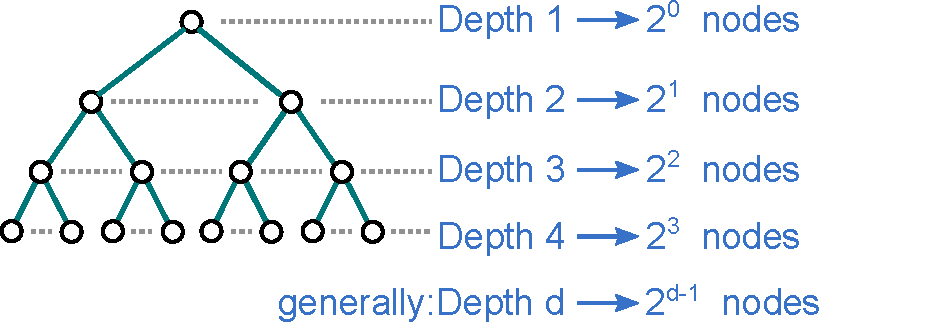
\includegraphics[width=0.7\textwidth]{Rolfs-Images/depth-nodes.pdf}
  \end{tabl}\\
  Runtime of \textit{heapify} with depth of $d$:
  \begin{itemize}
    \item
      No costs at depth $d$ with $2^{d - 1}$ (or less) nodes.
    \item<2->
      In a full heap with depth $d$ are $2 \, d - 1$ non-root nodes.\\
      The cost for \textbf{sifting} with depth $1$ are $1 \, C$
      ({\color{Mittel-Blau}compare})\\
      or $2 \, C$ ({\color{Mittel-Blau}compare} and
      {\color{Mittel-Blau}swap}) $\Rightarrow$ we use \Mittelblau{$2\cdot C$} to simplify
  \end{itemize}%

\end{frame}



\begin{frame}{Runtime - Heapsort 3/6}
  \begin{tabl}
  \item Overall:
  \end{tabl}
      \begin{center}%
        \begin{tabular}{c|c|c|c}
          Depth:     & Nodes:    & Path length: & Costs per node:\\
          \hline
          $d - 1$    & $2^{d-2}$     & 1            & $\leq 2 \cdot C$\\
          $d - 2$    & $2^{d-3}$ & 2            & $\leq 3 \cdot C$\\
          $d - 3$    & $2^{d-4}$ & 2            & $\leq 4 \cdot C$\\
          $\vdots$   & $\vdots$  & $\vdots$     & $\vdots$ 
        \end{tabular}\\[3em]
\onslide<2->
       \quad \Mittelblau{$\displaystyle  T(d) \leq \sum^d_{i=2} C\cdot i \cdot 2^{d-i} $}

    \end{center}%
%\onslide<4->

\end{frame}
%-------------------------------------------------------------------------------

\begin{frame}{Runtime - Heapsort 4/6}
  \begin{itemize}
    \item
      Runtime for heapify: 
      \[\displaystyle
\color{Mittel-Blau}
      T(d) \leq\underbrace{  C \cdot \sum \limits^d_{i=2} \left(i \cdot 2^{d-i} \right)
     \leq C \cdot 2^{d + 1}}_{\text{see next slides}}
\]\vspace*{-1em}
    \item<2-> Hence: cost for heapify: \Mittelblau{$T(d) \leq C\cdot 2^{d+1}$}
    \item<3-> \textbf{But:} we want cost in relation to \Mittelblau{$n$}
    \item<4->  a binary tree of depth \Mittelblau{$d$} has \Mittelblau{$2^{d-1}\leq n$}\quad{}\textcolor{Mittel-Gruen}{\textbf{Why?}}
      \begin{center}
        \onslide<5-> 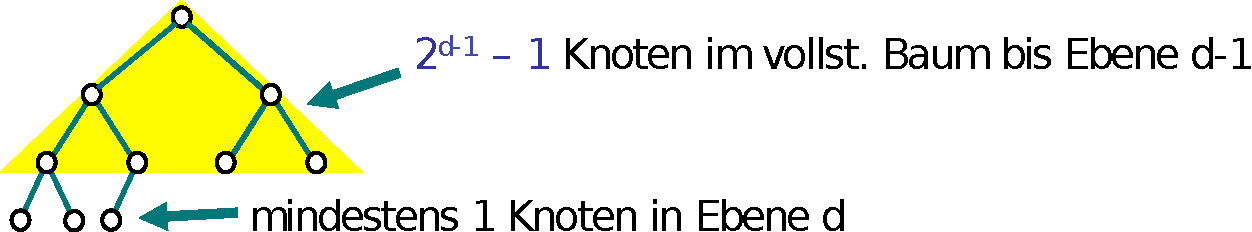
\includegraphics[width=0.8\textwidth]{Rolfs-Images/binary-tree-less-than-n.pdf} 
      \end{center}
    \item (Equation times \Mittelblau{$2^2$})  $\Rightarrow$ \Mittelblau{$2^{d-1}\cdot2^2 \leq 2^2\cdot n$}, so cost for heapify: 
      \begin{center}
$\color{Mittel-Blau}        T(n) \leq C\cdot4 \cdot n$
      \end{center}
  \end{itemize}
\end{frame}



\begin{frame}{Induction Proof}
  \begin{itemize}
    \item
      \textbf{We want to proof:} \vspace*{-1em}
      \begin{align*}
        \sum \limits^d_{i=1} \left(i \cdot 2^{d-i} \right) \leq &~ 2^{d+1}\\
        {\color{Hell-Gruen}A}(d) \leq &~ {\color{Hell-Gruen}B}(d)
      \end{align*}
we denote the left side with $A$, the right side with $B$    
\item<2->
      \textbf{Induction basis:}
      $d = 1$: \quad{} $A(1) \leq B(1)$
       \begin{align*}
        \sum \limits^d_{i=1} \left(i \cdot 2^{d-i} \right) \leq &~ 2^{d+1}\\
        \sum \limits^1_{i=1} \left(i \cdot 2^{1-i} \right) \leq &~ 2^{1+1}\\
        2^0 \leq &~ 2^2 ~{\color{Mittel-Blau}\checked}
      \end{align*}
  \end{itemize}
\end{frame}

%-------------------------------------------------------------------------------

\begin{frame}{Induction Proof for $ \sum^d_{i=1} \left(i \cdot 2^{d-i} \right) \leq ~ 2^{d+1}$}
  \textbf{Induction step:}
  $(d = d +1)$: \vspace*{-1em}
  \begin{displaymath}
   {\color{Hell-Gruen}A}(d) \leq ~ {\color{Hell-Gruen}B}(d) \hspace*{1.5cm}\Rightarrow \hspace*{1.5cm}
   {\color{Hell-Gruen}A}(d+1) \leq ~ {\color{Hell-Gruen}B}(d+1)    
  \end{displaymath}\vspace*{-2em}
    \begin{columns}
      \begin{column}{0.4\linewidth}
        \fbox{\begin{minipage}{0.95\linewidth}
        \textbf{Idea} write down right formula, and try to get \Mittelblau{$A(d)$} and \Mittelblau{$B(d)$} out of it.         
        \end{minipage}}
      \end{column}
        \begin{column}{0.5\linewidth}
            \onslide<2->          \begin{align*}
            % ----------------------------------------------------------------------
            \sum\limits^{d+1}_{i=1} \left(i \cdot 2^{d+1-i} \right)
           & \leq &~ 2^{d+1+1}\\
            % ----------------------------------------------------------------------
            2 \cdot \sum\limits^{d+1}_{i=1} \left(i \cdot 2^{d-i}
            \right)
            &\leq &~ 2 \cdot 2^{d+1}  \\
            % ----------------------------------------------------------------------
            2 \cdot \sum\limits^{d+1}_{i=1} \left(i \cdot 2^{d-i}
            \right)
            &\leq &~  2\cdot {\color{Hell-Gruen}B}(d) 
          \end{align*}
        \end{column}
            \end{columns}\vspace*{-1.5em}
\hspace*{1.7cm}            \onslide<3->\begin{minipage}{0.6\linewidth}
          \begin{align*}
            2 \cdot \sum\limits^{d}_{i=1} i \cdot 2^{d-i} \  \ +\ \ 2\cdot (d+1)\cdot 2^{d-(d+1)}     & \leq &~ 2 \cdot {\color{Hell-Gruen}B}(d)           \\
                        2 \cdot {\color{Hell-Gruen}A}(d) + (d+1) & 
            \leq &~ 2 \cdot {\color{Hell-Gruen}B}(d)           
          \end{align*}
        \end{minipage}
        \begin{itemize}
        \item<4-> \textcolor{red}{\textbf{Problem: doesn't work}} \textbf{but claim still holds}
        \end{itemize}

\end{frame}
%-------------------------------------------------------------------------------

\begin{frame}{Induction Proof for $ \sum^d_{i=1} \left(i \cdot 2^{d-i} \right) \leq ~ 2^{d+1}$}
  \textbf{working proof:} show a \textcolor{Mittel-Gruen}{little bit stronger} claim
  \begin{displaymath}
\textcolor{Mittel-Blau} \sum^d_{i=1} \left(i \cdot 2^{d-i} \right) \leq \textcolor{Mittel-Gruen}  2^{d+1} -d -2~ \textcolor{Mittel-Blau} \leq ~ 2^{d+1}
  \end{displaymath}
  \begin{itemize}
  \item<2-> \textbf{Advantage:} gives a stronger induction assumption
    \begin{center}
      \textcolor{Mittel-Gruen} \Rightarrow{} exercise
    \end{center}
  \end{itemize}
\end{frame}

%-------------------------------------------------------------------------------

%  \begin{frame}{Induction - Example 2}
%   \textbf{Induction step:}
%   $(d = d +1)$:
%   \begin{align*}
%     \sum\limits^{d+1}_{i=1} \left(i \cdot 2^{d-i} \right)
%     \leq &~ 2^{d+1}\\
%     %----------------------------------------------------------------------
%     \sum\limits^{d}_{i=1} \left(i \cdot 2^{d-i}\right)
%     + \left(d + 1\right) \cdot 2^{d - \left(d + 1\right)}
%     \leq &~ 2^{d+1}\\
%     %----------------------------------------------------------------------
%     \sum\limits^{d}_{i=1} \left(i \cdot 2^{d-i}\right)
%     + 2d + 2
%     \leq &~ 2^{d+1}\\
%     %----------------------------------------------------------------------
%    {\color{Hell-Gruen}A}(d) + 2d + 2
%    \leq &~ {\color{Hell-Gruen}B}(d) ~\textbf{\color{Mittel-Blau}\lightning}
%   \end{align*}
%   \begin{center}
%     \alert{Assumtion is still correct!}
%   \end{center}
% \end{frame}% Reset to Heapsort

%-------------------------------------------------------------------------------

\begin{frame}{Runtime - Heapsort 5/6}
  \begin{itemize}
    \item 
      Runtime for the other operations: \quad{} \raisebox{0.5\height}{\rlap{\begin{minipage}{0.4\linewidth}
  \tikzstyle{node}=[
  draw,
  circle,
  very thick,
  color=black,
  fill=white,
]%
%
\tikzstyle{node_filled}=[
  draw,
  circle,
  very thick,
  color=black,
  fill=orange!50!yellow
]%
%
\tikzstyle{node_leaf}=[
  draw,
  circle,
  very thick,
  color=black,
  fill=green!50!white,
]%
%
\tikzstyle{path}=[
  draw,
  line width=0.25em,
  color=orange!50!yellow!80!black
]%
%
\tikzstyle{path_normal}=[
  draw,
  very thick,
  color=black
]%
%
\begin{adjustbox}{width=\linewidth}
\begin{tikzpicture}[
  level/.style={
    sibling distance = 10.0em/#1,
    level distance = 3.5em
  }
]
\node [node_filled, label={[anchor=south]above:Root}] (root) {}
child [path_normal] {
  node [node] {}
  child {
    node [node] {}
    child {node [node_leaf, label={[anchor=east]left:Leaves}] {}}
    child {node [node_leaf] {}}
  }
  child {
    node [node] {}
    child {node [node_leaf] {}}
    child {node [node_leaf] {}}
  }
}
child [path] {
  node [node_filled] {}
  child {
    node [node_filled] {}
    child [path_normal] {node [node_leaf] {}}
    child {node [node_filled] {}}
  }
  child [path_normal] {
    node [node] {}
    child {node [node_leaf] {}}
    child {node [node_leaf] {}}
  }
};
\end{tikzpicture}
\end{adjustbox}
\end{minipage}}}\vspace*{-1em}
      \begin{itemize}
        \item<2->
          Constant costs for taking out $n \, \times$ maximum.
        \item<3->
          Maximum of $d$ steps repairing the heap $n$ times
        \item <4->
          Depth of heap at the start is $d \leq 1 + \log_2 n$ . \textcolor{Mittel-Gruen}{\textbf{why?}}
          \begin{center}
\onslide<5->            \color{Mittel-Gruen} $2^{d-1} \leq n \Rightarrow d-1 \leq \log_2 n \Rightarrow d \leq 1 + \log_2 n$
          \end{center}
            \item<6->
              Recall: the number of elements is decreasing
        \item<7->
              Hence: 
              $T(n) \leq n \cdot (1 +\log_2 n) \cdot C$
            \item<8-> the plus is ugly, but we can get:
              \begin{center}
                $T(n) \leq 2 \cdot n \, \log_2 n \cdot C$ \qquad (holds for $n > 2$).
              \end{center}
          \end{itemize}
  \end{itemize}
\end{frame}

%-------------------------------------------------------------------------------

\begin{frame}{Runtime - Heapsort 6/6}
  \textbf{Runtime costs:}
  \begin{itemize}
    \item
      Heapify: $T(n) \leq 4 \cdot n \cdot C$
    \item
      Remove: $T(n) \leq 2 \cdot n \, \log_2 n \cdot C$
    \item
      Total runtime: $T(n) \leq 6 \cdot n \, \log_2 n \cdot C$
    \item
      Constraints:
      \begin{itemize}
        \item
          Upper bound:
          $C_2 \cdot n \, \log_2 n \geq T(n)$ (for $n \geq 2$)
        \item
          Lower bound:
          $C_1 \cdot n \, \log_2 n \leq T(n)$ (for $n \geq 2$)
        \item
          $\Rightarrow$ $C_1$ and $C_2$ are constant
      \end{itemize}
  \end{itemize}
\end{frame}

\setcounter{subsubsection}{0}\section{Logaritms}

\begin{frame}{Base of Logaritms}
  \begin{block}{Logarithm to different bases:}
    $\log_a n = \dfrac{\log_b n}{\log_b a} = \log_b n \cdot \dfrac{1}{\log_b a}$
    
    The only difference is a constant coefficient $\frac{1}{\log_b a}$
  \end{block}
  \textbf{Examples:}
  \begin{itemize}
    \item
      \begin{math}
        \log_2 4
        = \log_{10} 4 \cdot \frac{1}{\log_2 10}
        = 0.602 \ldots \cdot 3.322 \ldots
        = 2 ~{\color{Mittel-Blau}\checked}
      \end{math}
    \item
      \begin{math}
        \log_{10} 1000
        = \log_{\mathrm{e}} 1000 \cdot \frac{1}{\log_{\mathrm{e}} 10}
        = \ln 1000 \cdot \frac{1}{\ln 10}
        = 3 ~{\color{Mittel-Blau}\checked}
      \end{math}
  \end{itemize}
\end{frame}

\appendix
\section*{\appendixname}
\subsection*{\LectureFurtherLiterature}
\input{Literature/Literature_\LectureLanguage}

\end{document}
